\documentclass[conference]{IEEEtran}
% Use to allow footnotes in the title.
%\IEEEoverridecommandlockouts

\ifCLASSOPTIONcompsoc
  % IEEE Computer Society needs nocompress option
  % requires cite.sty v4.0 or later (November 2003)
  \usepackage[nocompress]{cite}
\else
  % normal IEEE
  \usepackage{cite}
\fi

\usepackage{booktabs}
\usepackage{calc}
\usepackage{enumitem}
\usepackage{graphicx}
\usepackage{microtype}
\usepackage{tabularx}
\usepackage{url}
\usepackage[table]{xcolor}
\usepackage{xspace}

\newcommand*\rot{\rotatebox{90}}

\newcounter{tempstatlab}
\newcounter{tempstatlong}

\hyphenpenalty 10000
\exhyphenpenalty 10000

% To-do boxes
\newcommand*{\todo}[1]{{\color{red}\bf  TODO: #1}}

\begin{document}

\title{NCAA Men's Basketball Tournament Prediction}

\author{
  \textbf{Andrew Jacobson, Nate Jenkins, Trevor Smith, Joshua Stephens}\\
  CS 478, Winter 2018\\
  Department of Computer Science\\
  Brigham Young University\\
}
\maketitle

% comment this out for accepted papers - inserts page numbers for submission
\thispagestyle{plain}
\pagestyle{plain}

%% Page limite EuroUSEC - 10 pages body, 20 pages max

\begin{abstract}
Predicting the outcomes of the NCAA Men's Basketball Tournament has long fascinated many individuals.
We applied numerous machine learning models to the task, using season statistics and prior tournament data to predict future winners.
We find that a team's seeding dominates the decision making process.
Further features from a team's season statistics can be used to slightly improve prediction accuracy.
Upsets are particularly also particularly difficult for our chosen machine learning algorithms to predict.
\end{abstract}

\section{Introduction}
\todo{Finish Introduction}

Predicting the outcome of sporting events has been an interesting topic for some time.
People's interest in such events is manifest in activities like sports betting and fantasy teams.
One of the most popular prediction games is creating brackets for the NCAA Men's Basketball Tournament, often referred to as March Madness.

This particular tournament invites the believed 64 best teams to compete to determine the season's final champion.
These 64 teams play a combined total of 63 games.
This yields a total of over 9.2 Quadrillion possible brackets.
The odds of selecting a perfect bracket are so small that every year Warren Buffett promises to award any individual to do so \$1,000,000 per year for the rest of their life.

This extremely large space means that some sort of reasoning must be used to select a competitive bracket.
Human intuition usually has bias towards certain aspects of the selection.

Our project wanted to see what accuracy a machine is capable of when selecting a bracket.
To do this, we used a variety  of machine learning algorithms in combination with season and tournament statistics since 2003.

To quickly summarize our results:
\begin{enumerate}
	\item \textbf{Team Seeding is Important}: Due to the structure of seeded tournaments, better teams should win with much more regularity.
	\item \textbf{Season Statistics have an Minor Impact}: Including raw season statistics for individual teams can help improve accuracy, however, these statistics are the basis for seeding and typically only provide minimal improvements.
\end{enumerate}
\section{Methodology}

\subsection{Data Collection}
We collected our data from an online database from Kaggle\footnote{https://www.kaggle.com/c/mens-machine-learning-competition-2018/data}
This dataset provided season statistics for each NCAA basketball team since 2003.
We also acquired expert rankings from ESPN\footnote{http://www.espn.com/mens-college-basketball/rpi} and Kaggle.

This raw data was not organized in a way that allowed for accurate training models.
This was primarily due to team stats and records being organized by winning and losing team.
This caused the learning model to always select the winning team, since the winning teams stats were always input in the same places.
To rectify this, we had to randomly shuffle the wininng and losing teams into teams labled A and B and they classify the output as either A or B winning.

From this processed data, we used a number of combinations to see what different data sets would allow for prediction.
We primarily focused on three groups of data. 
First, we wanted to focus on exclusively the seeding as a baseline accuracy that we would strive to beat.
Next, we looked at several of the prominent ranking algorithms such as RPI and KenPom to see how well a community of ranking algorithms could do.
Then, we looked at a set of season statistics that we organized for each team. 
Finally, we combined these three datasets together to take advantage of all of our data.

\subsection{Learning Process}
We wanted to be able to effectively use all of the techniques that we had used in class to train and test our data.
A nice solution for this was to use the Python library sklearn which provides a nice high level abstraction.
With this library, we were able to structure our training to include all of the following supervised learning models: logistic regression, decision tree, naive bayes, neural network, random forest, boosted forest, gaussian process, k-nearest neighbor, support vector machine, and several ensembles.
We were able to structure our code to see results from all of these learners and make educated decisions on which models consistently performed the best and how we could then use ensembles of those models to further improve the results.
\section{Initial Results}
As mentioned in the previous section, we started by establishing a baseline accuracy by just using the seeding data.
Here are the results from each year and the average overall results.

\vspace{0.5cm}
\begin{tabular}{lc}
  \toprule
  Year & Accuracy\\
  \midrule
  2004 & 0.75\\
  2005 & 0.7187\\
  2006 & 0.6875\\
  2007 & 0.8125\\
  2008 & 0.7656\\
  2009 & 0.75\\
  2010 & 0.6875\\
  2011 & 0.6865\\
  2012 & 0.7313\\
  2013 & 0.7014\\
  2014 & 0.6716\\
  2015 & 0.7910\\
  2016 & 0.7313\\
  2017 & 0.7611\\
  All & 0.7170\\
  \bottomrule
\end{tabular}
\vspace{0.5cm}

So, initially we discovered that the seeding provided a good baseline with a pretty high standard. 
We also saw that the accuracy varies significantly from year to year. 
Furthermore, the potentially noticed that the accuracy has a small negative correlation with the year. 
We should also mention that each year used all the previous years as training data.
This meant that the later years were able to use more data to make their decisions.
In summary, it seems that it is getting harder and harder to predict the outcomes of games based on solely the seed.
Here is a picture of the seeding accuracies for each year in our dataset:

\begin{center}
  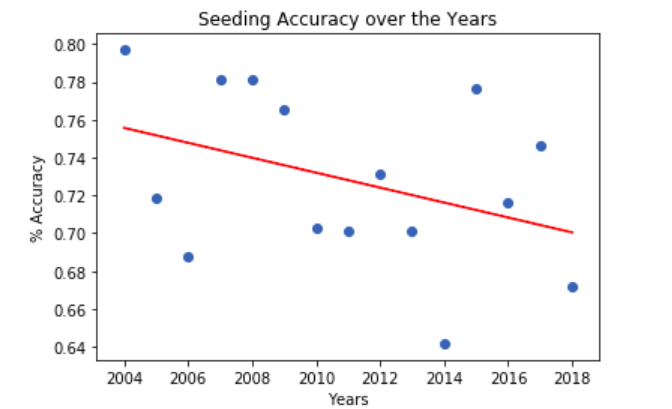
\includegraphics[width=9.5cm]{SeedingAccuracies.png}
\end{center}

Next, we looked at the ability of several top ranking systems to predict the tournament outcomes.
We found that 3 of the ranking systems seemed to outperform the others: RPI, KenPom, and SAG.
Since the seed is technically another ranking system, we included it in this section of data as well.
Here are the results for this set of data as well as how they compare to the baseline.

\vspace{0.5cm}
\begin{tabular}{c c c}
    \toprule
    Year & Accuracy & Difference\\
    \midrule
    2004 & 0.75 & +0.0000\\
    2005 & 0.7343 & +0.0156\\
    2006 & 0.6875 & +0.0000\\
    2007 & 0.8281 & +0.0156\\
    2008 & 0.8281 & +0.0625\\
    2009 & 0.7656 & +0.0156\\
    2010 & 0.6718 & -0.0157\\
    2011 & 0.6865 & +0.0000\\
    2012 & 0.7313 & +0.0000\\
    2013 & 0.6865 & -0.0149\\
    2014 & 0.6865 & +0.0149\\
    2015 & 0.7761 & -0.0149\\
    2016 & 0.7462 & +0.0149\\
    2017 & 0.7611 & +0.0000\\
    All & 0.7193 & +0.0023\\
    \bottomrule
\end{tabular}
\vspace{0.5cm}

These initial results helped us establish a baseline accuracy for predicting march madness outcomes.
As we saw in past years and particularly in this year, the tournament prediction is dominated by guessing the correct upsets.
With this in mind, we were interested in trying some new features, making combinations of our features, and enhancing the features that we have.
\section{Feature Enchancement}

Having established this baseline accuracy of about 71\% using the seeds, we wanted to improve our accuracy by performing some feature improvements. 
We started by using statistics gained over each team’s regular season. 
Then we combined those features with the features from the top ranking systems to try to take advantage of all our data. 
In both cases we used some a wrapper algorithm for feature selection with each of our prediction algorithms to try to get the best combinations for a feature set.

First, we wanted to use the seasonal statistics to see if we could improve on our baseline accuracy.
The seasonal statistics included the following features: number of wins, number of losses, averages per game for points, shots made, shots attempted, three-point shots made, three-point shots attempted, rebounds, assists, turnovers, steals, blocks, and personal fouls.
Here are the results from each year and the average overall results compared to our baseline accuracies by seed using this new feature set. 

\vspace{0.5cm}
\begin{tabular}{c c c}
    \toprule
    Year & Accuracy & Difference\\
    \midrule
    2004 & 0.7187 & -0.0313\\
    2005 & 0.6875 & -0.0312\\
    2006 & 0.7187 & +0.0312\\
    2007 & 0.7812 & -0.0313\\
    2008 & 0.7968 & +0.0312\\
    2009 & 0.7031 & -0.0469\\
    2010 & 0.6875 & +0.0000\\
    2011 & 0.6865 & +0.0000\\
    2012 & 0.7313 & +0.0000\\
    2013 & 0.7164 & +0.0150\\
    2014 & 0.6567 & -0.0149\\
    2015 & 0.7462 & -0.0448\\
    2016 & 0.7164 & -0.0149\\
    2017 & 0.7164 & -0.0447\\
    All & 0.7289 & +0.0019\\
    \bottomrule
\end{tabular}
\vspace{0.5cm}

We saw that there was little improvement on the baseline accuracy using seasonal statistics. 
Much like the results that we gained from using the top ranking systems mentioned in our initial results, there were years that had better accuracies, years that had worse accuracies, and years that had no change in accuracies. 
Overall, on all of the years we saw that there was less than 1\% on the increase of accuracy. 
This meant that adding these features had very little effect on the outcome of our predictions. 

We continued to tweak the seasonal statistics features by including certain combinations of them instead of adding all of them to the feature set. 
To do this we used a wrapper algorithm called recursive feature elimination. 
The goal was to select the optimal number of features by considering each set of features. 
Each iteration got the same results, about 72\% in the overall accuracy. 
There was no combination of features which resulted in an accuracy much larger than the initial accuracy gained by simply using only the seed.


\section{Final Results}

Our next step was to combine the seasonal statistic features with the top ranking systems features used in our initial results. 
We thought this would take advantage of all of our data and combine to result in greater accuracies than we have gained so far. 
Here are the results from each year and the average overall results compared to our baseline accuracies by seed using this new feature set.


\vspace{0.5cm}
\begin{tabular}{c c c}
    \toprule
    Year & Accuracy & Difference\\
    \midrule
    2004 & 0.8125 & +0.0625\\
    2005 & 0.7187 & +0.0000\\
    2006 & 0.7187 & +0.0312\\
    2007 & 0.7968 & -0.0157\\
    2008 & 0.7500 & -0.0156\\
    2009 & 0.7343 & -0.0157\\
    2010 & 0.7500 & +0.0625\\
    2011 & 0.6716 & -0.0149\\
    2012 & 0.6865 & -0.0448\\
    2013 & 0.6567 & -0.0447\\
    2014 & 0.6865 & +0.0149\\
    2015 & 0.7611 & -0.0299\\
    2016 & 0.7164 & -0.0149\\
    2017 & 0.7761 & +0.0150\\
    All & 0.7217 & +0.0047\\
    \bottomrule
\end{tabular}
\vspace{0.5cm}

We again saw little improvement on the baseline accuracy using this new feature set. 
Even though we used all of the data and many features, the overall accuracy increased less than 1\% compared to the baseline accuracy. 

We again tried using recursive feature elimination to get the best combinations of features for each of our algorithms. 
Using the entire data set full of each feature, we still saw that the overall accuracy did not increase more than 72\%. 

We were not thrilled about these results and we wanted to do better than 72\%. 
We tried to think of ways to increase our accuracy and we thought that they only way we could do this was to try to predict upset games in a creative way.
\section{Discussion}
\subsection{Importance of Seed}
\subsection{Dependance on Season Statistics}
\section{Future Work}
Our final week or so of effort was devoted to exploring the probabilities of upsets. 
These two sections talk about our efforts to calculate the probability of an upset and how that can lead into a future project.

\subsection{Probabilistic Upsets}
Because we were unsuccessful in improving the model beyond the accuracy achieved using the seeding data we collected, we decided to explore the possibility of predicting the most likely upsets. 

In order to do so, we decided to define upsets as games in which the seeding between both teams differed by 5 or more seeds. 
The intention of this sub setting was to focus on the features that might best predict upsets. 
Additionally, upsets are a relatively rare occurrence in these games. 
In fact, in games where the seed differed by at least five games, upsets occurred with a frequency of roughly 21\%.
Because the dataset was skewed towards few upsets, the data was undersampled to create a dataset with 50\% upsets and 50\% non-upset games. 
Again, this was done in hopes of creating a dataset that is more likely to find attributes that are predictive of upset games. 

Using this data, a logistical regression model was fit to predict upsets. 
The predictive accuracy on a test set from original data yielded an accuracy of roughly 73\%. 
Although this accuracy is not very high, the logistic regression model allowed for a probabilistic output. 
In other words, we were able to get a list of the most likely upsets probability wise. 

These probabilities offer the potential of adding some picks for upsets to one’s bracket that our other models would not have chosen. 
Because bracket prediction is so difficult, it is worthwhile to add some potential upsets to a bracket selected by this model. 
By adding these upsets to a bracket, the chances of winning a bracket challenge will increase. 

This also may be the subject of future work, as the real challenge in creating good brackets is to figure out which upsets are most likely. 
In the future it would certainly be worthwhile to try more models and different techniques of finding the most likely upsets in the tournament.

\subsection{Bracket Creation}
Our next step from these small tests would be to try to create brackets that were randomly generated using our upset predictor and see if we can randomly pick the correct upsets.
The mean idea is that predicting the most likely victor for all the games, even when 100\% correct, won't produce a bracket that wins in any of the competitions.
However, we would be interested to see if a set of 100 brackets, each with an intelligent set of upsets, would have a few brackets that more accurately predicted the outcomes of the tournament.

\section{Conclusion}
Predicting a perfect bracket, given the 9.2 quadrillion permutations, remains difficult, even with the aid of modern machine learning models.
To reiterate our findings included:
\begin{enumerate}
	\item Baseline prediction using only seeding data and choosing the higher seed to win generally yields around 70\% accuracy.
	\item Improved predictions can be made by using team statistics and rankings, though these improvements are generally only by a few percentage points.
	\item If a perfect bracket is to be found, the upsets must be inserted and can be better guessed using probabilistic methods.
\end{enumerate}

While the perfect bracket may remain a guessing game, producing a set of strong brackets to compete against friends, family, and colleagues with is certainly obtainable.



\bibliographystyle{IEEEtran}
\bibliography{main}
\section{References}
\begin{enumerate}
	\item Season Data. Retrieved February 20, 2018, from https://www.kaggle.com/c/mens-machine-learning-competition-2018/data
	\item Team Rankings. Retrieved February 20, 2018, from http://www.espn.com/mens-college-basketball/rpi
\end{enumerate}

\end{document}
